%##noBuild
\newpage
\section{Funkcje}

\subsection{UCZESTNICY WYCIECZKI}
%09-conference-logic
uczestnicy\_wycieczki (id\_wycieczki), procedura ma zwracać podobny zestaw danych jak
widok wycieczki\_osoby.

\subsubsection{TYPE UCZESTNICY WYCIECZKI}
\begin{verbatim}
CREATE OR REPLACE TYPE TYPE_UCZESTNICY_WYCIECZKI AS OBJECT (
  ID_OSOBY NUMBER,
  IMIE     VARCHAR(50),
  NAZWISKO VARCHAR(50)
);
\end{verbatim}

\subsubsection{TABLICA UCZESTNICY WYCIECZKI}
\begin{verbatim}
CREATE OR REPLACE TYPE TAB_UCZESTNICY_WYCIECZKI AS TABLE OF TYPE_UCZESTNICY_WYCIECZKI;
\end{verbatim}


\subsubsection{FUNKCJA UCZESTNICY WYCIECZKI}
\begin{verbatim}
CREATE OR REPLACE FUNCTION UCZESTNICY_WYCIECZKI(ID IN NUMBER)
  RETURN TAB_UCZESTNICY_WYCIECZKI PIPELINED
AS
  BEGIN
    FOR X IN (SELECT R.ID_OSOBY, O.IMIE, O.NAZWISKO, R.ID_WYCIECZKI
              FROM REZERWACJE R
                     INNER JOIN OSOBY O ON O.ID_OSOBY = R.ID_OSOBY
              WHERE R.ID_WYCIECZKI = ID)
    LOOP
      PIPE ROW (TYPE_UCZESTNICY_WYCIECZKI(X.ID_OSOBY, X.IMIE, X.NAZWISKO));
    END LOOP;
  END;
\end{verbatim}

\begin{minipage}{0.40\textwidth}
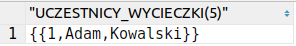
\includegraphics[width=\linewidth]{./images/uczestnicy_wycieczki.png}
\end{minipage}

\subsection{REZERWACJA OSOBY}
rezerwacje\_osoby(id\_osoby), procedura ma zwracać podobny zestaw danych jak widok
wycieczki\_osoby

\subsubsection{TYPE REZERWACJE OSOBY}
\begin{verbatim}
CREATE OR REPLACE TYPE TYPE_REZERWACJE_OSOBY AS OBJECT (
  NR_REZERWACJI NUMBER
);
\end{verbatim}

\subsubsection{TABLICA REZERWACJE OSOBY}
\begin{verbatim}
CREATE OR REPLACE TYPE TAB_REZERWACJE_OSOBY AS TABLE OF TYPE_REZERWACJE_OSOBY;
\end{verbatim}

\subsubsection{FUNKCJA REZERWACJE OSOBY}
\begin{verbatim}
CREATE OR REPLACE FUNCTION REZERWACJE_OSOBY(ID NUMBER)
  RETURN TAB_REZERWACJE_OSOBY PIPELINED
AS
  BEGIN
    FOR X IN (SELECT R.NR_REZERWACJI
              FROM REZERWACJE R
                     INNER JOIN OSOBY O ON R.ID_OSOBY = O.ID_OSOBY
              WHERE O.ID_OSOBY = ID)
    LOOP
      PIPE ROW (TYPE_REZERWACJE_OSOBY(X.NR_REZERWACJI));
    END LOOP;
  END;
\end{verbatim}

\begin{minipage}{0.40\textwidth}
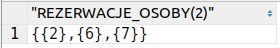
\includegraphics[width=\linewidth]{./images/rezerwacje_osoby.png}
\end{minipage}\\
Pomocniczo tabela rezerwacji:\\ 
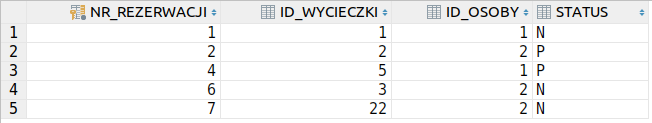
\includegraphics[width=\linewidth]{./images/przyszle_rezerwacje_osoby_rezerwacje.png}

\subsection{PRZYSZŁE REZERWACJE OSOBY}
przyszle\_rezerwacje\_osoby(id\_osoby)

\begin{verbatim}
CREATE OR REPLACE FUNCTION PRZYSZLE_REZERWACJE_OSOBY(ID NUMBER)
  RETURN TAB_REZERWACJE_OSOBY PIPELINED
AS
  BEGIN
    FOR X IN (SELECT R.NR_REZERWACJI
              FROM REZERWACJE R
                     INNER JOIN OSOBY O ON R.ID_OSOBY = O.ID_OSOBY
                     INNER JOIN WYCIECZKI W ON R.ID_WYCIECZKI = W.ID_WYCIECZKI
                   WHERE O.ID_OSOBY = ID AND W.DATA > (SELECT CURRENT_DATE FROM DUAL)
              )
    LOOP
      PIPE ROW (TYPE_REZERWACJE_OSOBY(X.NR_REZERWACJI));
    END LOOP;
  END;
\end{verbatim}
\begin{minipage}{0.40\textwidth}
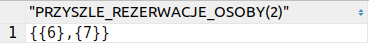
\includegraphics[width=\linewidth]{./images/przyszle_rezerwacje_osoby.png}
\end{minipage}\\
Pomocniczo tabela rezerwacji:\\
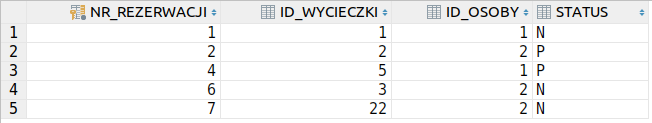
\includegraphics[width=\linewidth]{./images/przyszle_rezerwacje_osoby_rezerwacje.png}
Pomocniczo tabela wycieczki:\\
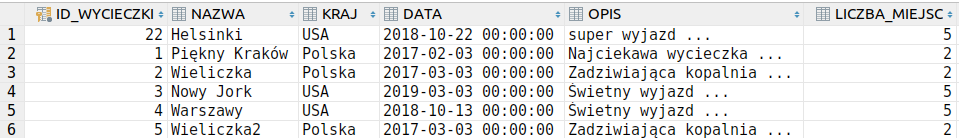
\includegraphics[width=\linewidth]{./images/przyszle_rezerwacje_osoby_wycieczki.png}
\subsection{DOSTĘPNE WYCIECZKI}
dostepne\_wycieczki(kraj, data\_od, data\_do)

\subsubsection{TYPE DOSTĘPNE WYCIECZKI}
\begin{verbatim}
CREATE OR REPLACE TYPE TYPE_DOSTEPNE_WYCIECZKI AS OBJECT (
  KRAJ VARCHAR(50),
  DATA DATE
);
\end{verbatim}

\subsubsection{TABLICA DOSTĘPNE WYCIECZKI}
\begin{verbatim}
CREATE OR REPLACE TYPE TAB_DOSTEPNE_WYCIECZKI AS TABLE OF TYPE_DOSTEPNE_WYCIECZKI;
\end{verbatim}

\subsubsection{FUNKCJA DOSTĘPNE WYCIECZKI}
\begin{verbatim}
CREATE OR REPLACE FUNCTION DOSTEPNE_WYCIECZKI(KRAJ VARCHAR2, DATA_OD DATE, DATA_DO DATE)
  RETURN TAB_DOSTEPNE_WYCIECZKI PIPELINED
AS
  BEGIN
    FOR X IN (SELECT W.KRAJ, W.DATA
              FROM WYCIECZKI W
              WHERE W.LICZBA_MIEJSC -
                    NVL(
                      (SELECT COUNT(*) FROM REZERWACJE R WHERE W.ID_WYCIECZKI = R.ID_WYCIECZKI GROUP BY R.ID_WYCIECZKI),
                      0) > 0
                AND ((SELECT CURRENT_DATE FROM DUAL) < W.DATA)
                AND (W.DATA BETWEEN DATA_OD AND DATA_DO)
                AND W.KRAJ = KRAJ)
    LOOP
      PIPE ROW (TYPE_DOSTEPNE_WYCIECZKI(X.KRAJ, X.DATA));
    END LOOP;
    RETURN;
  END; 
\end{verbatim}

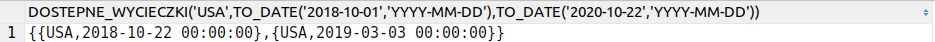
\includegraphics[width=\linewidth]{./images/dostepne_wycieczki_funkcja.png}